\documentclass[a4paper]{article}

\usepackage{hyperref}
\usepackage{graphicx}
\usepackage{amsmath}
\usepackage{amsthm}
\usepackage{amsfonts}

\newtheorem{algorithm_def}{Algorithm}[section]
\newtheorem{definition}{Definition}[section]
\newtheorem{lemma}{Lemma}[section]
\newtheorem{theorem}{Theorem}[section]
\newtheorem{corollary}{Corollary}[section]

\DeclareMathOperator*{\argmin}{arg\,min}
\DeclareMathOperator*{\argmax}{arg\,max}

%opening
\title{Robot on icy surface \\ {\small CS6244 Robot Motion Planning \& Control (Prof David Hsu)} }
\author{
  Jahja, Irvan\\
  {\small A0123879R} \\ \texttt{dolphinigle.mailbox@gmail.com}
  \and
  Nguyen, Rang H. M.\\
  {\small A0123879R} \\ \texttt{dolphinigle.mailbox@gmail.com}
}

\begin{document}

\maketitle

\section{Motivation}
% * Provide an intuitive description of the problem domain. Describe the motivation and potential applications.
A car-like robot was dropped on the northern pole few days ago. It has collected various
data on the north pole, and now is ready for pickup at a specific destination,
and with a specific orientation. However, due to global warming, pool of water
forms on the icy surface, and falling into any of them spells certain disfunction
for the robot. Furthermore, icy surface make it very hard for the robot to
follow paths exactly, rendering normal techniques to solve the non-holonomic
motion planning less useful. How are we going to save the robot?

Enter this project. Our algorithm is able to guide the robot to its destination
reliable and, if the robot slips, correct its path, all in real-time. Our algorithm
is able to guide the robot despite uncertainty in its movement -- the preceeding
paragraph gives one such surface that may have unignorable uncertainty.

This project aims to devise such an algorithm, and demonstrates exactly why
we are not allowed to ignore uncertainty in the experiments.

\section{Problem statement}
% * State the technical problem formally. 

\subsection{Configuration space}
We consider a point robot moving on a two dimensional space $\mathbb{R}^2$.
The robot position is denoted by its coordinates $(x, y)$. We restrict the space
to $[0\ldots1, 0\ldots1]$ (that is, we must have $0 \le x \le 1$ and $0 \le y \le 1$).
The robot also has an orientation, denoted by $\theta$. Thus, the robot's
configuration is $(x, y, \theta)$ of dimension $3$.

In addition, there are polygonal obstacles lying on the space. The robot
are not allowed to collide with these obstacles -- doing so results in the
failure of the execution. In addition, the robot is also not allowed to go
past the boundaries of the space. More specifically, whenever the robot's
configuration is within an obstacle or outside the boundaries of the field,
the robot's execution failed.

We assume that the robot is able deduce its current configuration space at
any time -- that is, we assume perfect sensing and knowledge of the configuration space
and the configuration of the robot.

\subsection{Robot movement and non-holonomic constraint}
The robot's movement is governed by a car-like non-holonomic law -- the robot
has a length of $L$ and has a maximum steering distance of $\theta_{\text{max}}$.
The robot can freely adjust its steering distance as long as its absolute
value does not exceed $\theta_{\text{max}}$.  When the
robot's steering angle is at $\alpha$, then the turning radius of the robot
is $L / \sin(\alpha)$, meaning that if the robot steers it with angle of $\alpha$,
it will roughly follow an arc of a circle of radius $L / \sin(\alpha)$.

For simplicity, we assume that the robot do not have the capabilities to move
backwards. Extending the algorithm to support this movement is immediate, but
does not give interesting results.

\subsection{Uncertainty}
In addition, the robot is unable to execute commands perfectly. The coordinates
and orientation of the robot suffers from a noise sampled from an unknown distribution
with known variance (in practice, we can probably measure this variance).
Thus, when we perform integration over the length of the path, by the central
limit theorem, this value is approximately normal. Thus, we model the noise
using normal distribution with variance $\sigma^2$ for the coordinates and
$\sigma_\theta^2$ for the orientation.

\subsection{Objective}
The objective of the robot is to approximately reach a specific location with a
specific orientation. More exactly, the robot is given a goal configuration
$(x_g, y_g, \theta_g)$, and the robot must reach a configuration $(x, y, \theta)$
such that $|\theta - \theta_g| < \delta$ and $|(x, y)^2 - (x_g, y_g)^2| < T$,
for a threshold $T$ and orientation tolerance $\delta$. Note that the probability
of the robot reaching exactly the configuration $(x_g, y_g, \theta_g)$ might be
zero due to uncertainty in movement.

\section{Algorithm description}
% * Present your algorithm. Describe the input and output if necessary. 
We model the problem using the Markov Decision Process, and use value iteration
to find the optimal actions at each step.
The values of the various parameters associated with the algorithm is
summarized in Figure~\ref{f:notations}.

\subsection{Abstract model}

The markov model of our problem is as follows. Each state in the markov model
would be a configuration in the configuration space. At each state, the robot's
action constitutes of setting the steering angle. Because of the noise, however,
the steering angle does not lead deterministically to the next state.

\subsection{Discretization}
Markov Decision Process assumes a finite number of states and a finite number
of actions. Without discretization, there is an infinite number of
configurations and infinite number of actions. Thus, we discretize the configuration
space and the actions as follows.

\subsubsection{Configuration discretization}
For the space, we discretize each of the axis of the coordinates into $n$
equal-width spaces. We further discretize the angle into $m$ equally-spaced
intervals. Thus, each state is a square cell of $\mathbb{R}^2$ and an orientation
range.

We consider a square cell to be bad if it intersects with an obstacle. Thus, with
very small values of $n$, it might be possible that all square cells are considered
bad, and thus we suggest using values of $n$ that is reasonably high. A rough
guideline is as follows: if the size of the smallest gap is $x$, then we
suggest using $n \ge 2/x$. If all the obstacles are axis aligned, then this
would guarantee that there exists a sequence of adjacent non-bad path from the
start to the goal states if there exists such a path in the non-discretized space.

\subsubsection{Action discretization}
For simplicity, we only consider three possible actions: steer all the way
to the left, steer all the way to the right, or steer straight. That is,
the only three steering angles we consider are $\{-\theta_\text{max}, 0, \theta_\text{max}\}$.

\subsection{Markov model}
The markov decision process has the following elements:
\begin{itemize}
  \item S (the set of states): corresponds to each of the discretized cells.
  \item A (the set of actions): $\{-\theta_\text{max}, 0, \theta_\text{max}\}$.
  \item T (the transition function): will be described in section~\ref{sec:t}.
  \item R (the reward function): will be described in section~\ref{sec:r}.
\end{itemize}

In addition, we use an infinite horizon model with discount factor of $\eta$.

\subsubsection{Action configuration transitition}
\label{sec:t}
To model the transition probability function $T(s, a, s')$ (probability of
reaching state $s'$ when executing action $a$ in state $s$), we do the following.
Each action is taken as if it were to be executed until a distance of $\delta$
is travelled. To model the noise, at the projected end of the movement, we
shift the configuration coordinates by a normal distribution with variance
$\sigma^2$ for the coordinates and $\sigma_\theta^2$ for the orientation.

More specifically, $T(s, a, s')$ is computed as follows. Let $(x, y)$ be the
center of the cell of $\mathbb{R}^2$ of state $s$. Consider when the robot
align its steering angle to $a$ until he walked a distance of $\delta$. He
will arrive in another point $(x', y')$, and with a new orientation $\theta'$.
For each $a \in \{x', y', \theta'\}$, consider the normal distribution
with mean equal to $a$ and its corresponding variance. We calculate the probability
that each of these distributions fall under the state $s'$, and multiply all
of them together to obtain $T(s, a, s')$.

\subsubsection{Reward function}
\label{sec:r}
Intuitively, we would like the reward function to deter the robot from entering
obstacles, and reward it if it reaches the goal configuration. More formally,
we give the robot positive reward ($r_g$) if it reaches the goal, and a large negative
reward $r_i$ if it falls to ice. Thus, the reward is actually based on would-be state,
that is, $R(s, a, s')$. Thus, we convert this to $R(s, a)$ by multiplying the
reward by the probability of reaching the state, that is:

\[ R(s, a) = \sum_{s' \in S} T(s, a, s') \cdot R(s, a, s') \]

\section{Results and discussions}
% * Present the theoretical analysis, experiment results, comparison, etc., as applicable.

The values of the parameters used for testing is summarized in Figure~\ref{f:notations}.
We use the value displayed unless stated otherwise.

\begin{figure}
\label{f:notations}
\caption{Various notations we use and its default values for the experiments}
\begin{tabular}{ l | l | l }
  Symbol & Description & Value \\ \hline \hline
  $n$ & Grid resolution & 20 \\ \hline
  $m$ & Orientation resolution & 16 \\ \hline
  $L$ & Length of the car & 0.1 \\ \hline
  $\theta_{\text{max}}$ & Maximum turning angle & $\pi / 4$ \\ \hline
  $\delta$ & Length of a single step of execution & $2^{0.5} / n$ \\ \hline
  $r_g$ & Reward upon reaching the goal & 100 \\ \hline
  $r_i$ & Reward if fall into ice & -10000 \\ \hline
  $\eta$ & Discount factor & 0.95 \\ \hline
\end{tabular}
\end{figure}

The default configuration of obstacles that we use is depicted in Figure~\ref{f:b_shortest}.

\begin{figure}
\label{f:b}
\caption{The default configuration used in the subsequent tests. The starting
  configuration is on the bottom left, facing northeast. The goal configuration
  is on the top right, facing east. The configuration consists
  of large corridors and a small corridor that offers shortcut from the start
  and goal configurations. Assuming no noise, the shortest path from the start
to the goal configuration we find is depicted in the figure as well.}
\centerline{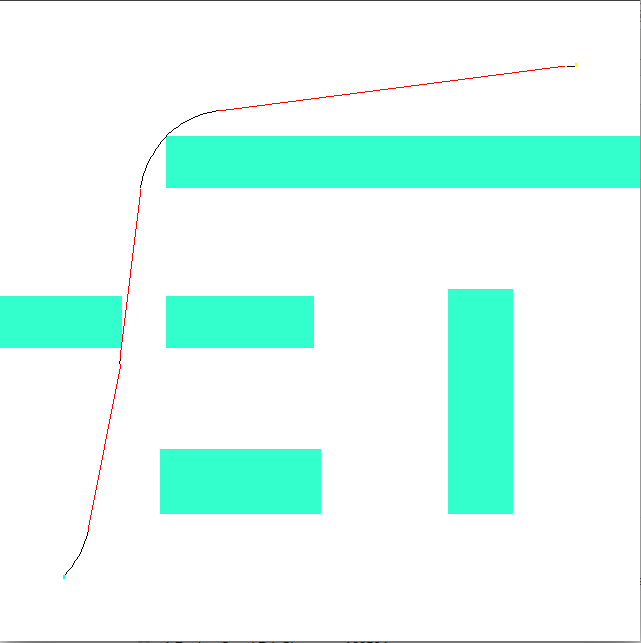
\includegraphics[width=5cm]{b_shortest.png}}
\end{figure}

\subsection{Figure description}
Figure~\ref{f:b} shows the result of running the algorithm on the default
configuration with default values.

\begin{figure}
\label{f:b}
\caption{Result of running the algorithm on the default configuration with default values.
Amongst 1000 executions, 780 of them successfully reached the goal configuration.
The value iteration terminated after 150 iterations.}
\centerline{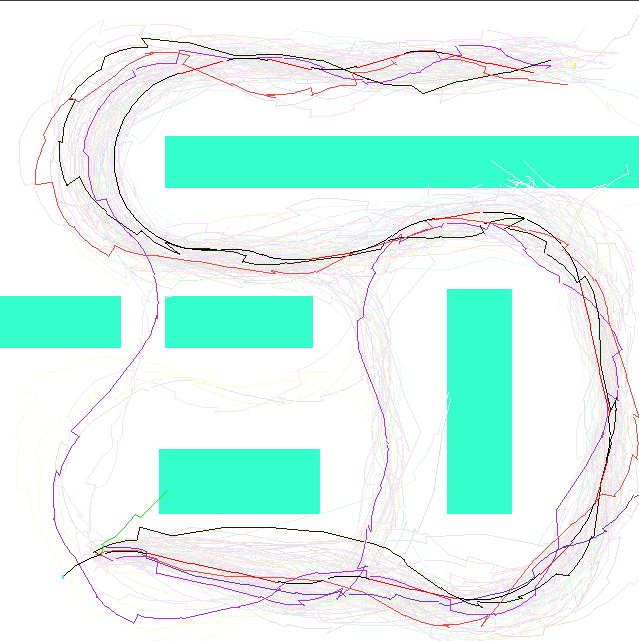
\includegraphics[width=5cm]{b.png}}
\end{figure}

In all the figures, including Figure~\ref{f:b}, we adopt the following notations.
The alternating black and red line is the path the robot would follow if
all of its movements are exact. The light grey paths depicts multiple paths
that were generated. In addition, there are 5 other bright colored paths that
are chosen randomly from all the generated paths. The paths may not seem continuous
because we discretize the noise so that it only happens between paths of length
$\delta$.

\subsection{Default value discussion}
In Figure~\ref{f:b}, we make the following observations. The path chosen is
significantly different from the shortest path -- here, the algorithm prefer
to drive the robot to follow the large corridor on the right, even though
the path is longer. This is in line with our intuition that, since the deterrant
of falling into ice is high, it is more beneficial to take the less risky way,
even though it makes the reward somewhat smaller due to applying the discount
factor more.

More interestingly, the appearance of uncertainty makes the movement much more
diverse. There seems to be two major paths: through the center corridor or
through the right corridors. We note that whenever the noise affects the robot
such that it goes "off track", instead of correcting its original track, the
robot may instead follow a different track. This is good as it follows
intuition -- backtracking to the original path may be more dangerous
than following the new path. For example, in the purple path, the robot is
quite affected by the noise that it have to make two different paths: the first
happens on the center intersection, where instead of going straight, it instead
decides to go down since its orientation points too sharply to the south. The
second one happens near the narrow corridor on the left, where its orientation
is affected so much that it points too north, and thus the robot decides to
brace through the narrow corridor instead (and succesfully so).

As an additional observation, we observed that most of the failure occurs on the
right corridor when turning. It seems that it is for this reason that the path
tries to follow the larger corridor on the right, because it requires larger degree
of error before failing, therefore minimizing the chance of failure. However,
an alternative, less pleasant, reasoning of choosing the right corridor might
be that the algorithm tries to make the failure occurs as late as possible,
instead of minimizing the probability of failure -- which is an unfortunate side
effect of this algorithm.

\subsection{Effect of discretization resolution}
The following results seems to suggest that increasing the resolution makes the algorithm
succeed more often.

We ran two additional experiments in addition to the one using the default
values. The result is summarized in Figure~\ref{f:resolution}.
The individual results for $n=15$ and $n=10$ are depicted in Figure~\ref{f:midres} and Figure~\ref{f:lowres},
respectively. We were unable
to succesfully run the algorithm with a resolution significantly higher than
$20$, due to the computer running out of memory (for storing the MDP model).

\begin{figure}
\label{f:resolution}
\caption{Effect of resolutions. Time of execution excludes the time required
         to generate the transition function of the MDP}
\begin{tabular}{ l | l | l | l }
  $n$ & $m$ & Success rate & Time of execution \\ \hline \hline
  $20$ & $16$ & $0.780$ & $90$ seconds \\ \hline
  $20$ & $12$ & $0.780$ & $90$ seconds \\ \hline
  $20$ & $8$ & $0.780$ & $90$ seconds \\ \hline
  $15$ & $16$ & $0.124$ & $18$ seconds \\ \hline
  $15$ & $12$ & $0.124$ & $18$ seconds \\ \hline
  $15$ & $8$ & $0.124$ & $18$ seconds \\ \hline
  $10$ & $16$ & $0.112$ & $6$ seconds \\ \hline
  $10$ & $12$ & $0.112$ & $6$ seconds \\ \hline
  $10$ & $8$ & $0.122$ & $3$ seconds \\ \hline
\end{tabular}
\end{figure}

\begin{figure}
\label{f:b}
\caption{Default configuration with $n=15$, and $m=12$}
\centerline{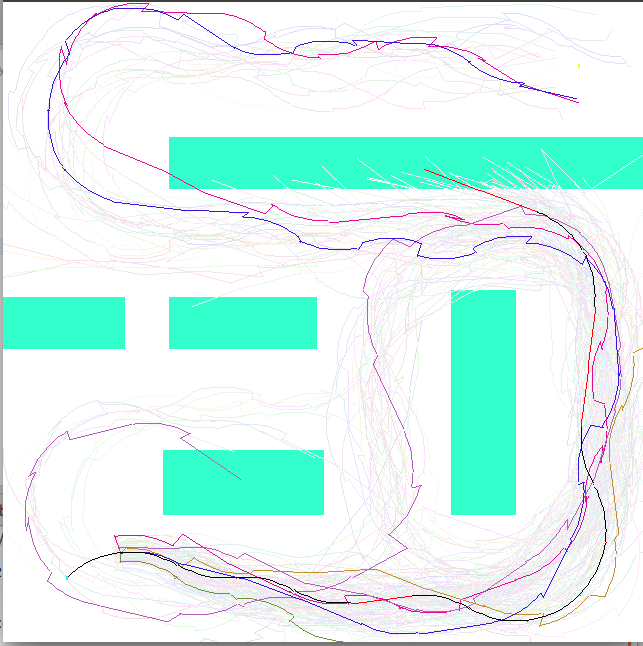
\includegraphics[width=5cm]{b_medres.png}}
\end{figure}

\begin{figure}
\label{f:b}
\caption{Default configuration with $n=10$, and $m=8$}
\centerline{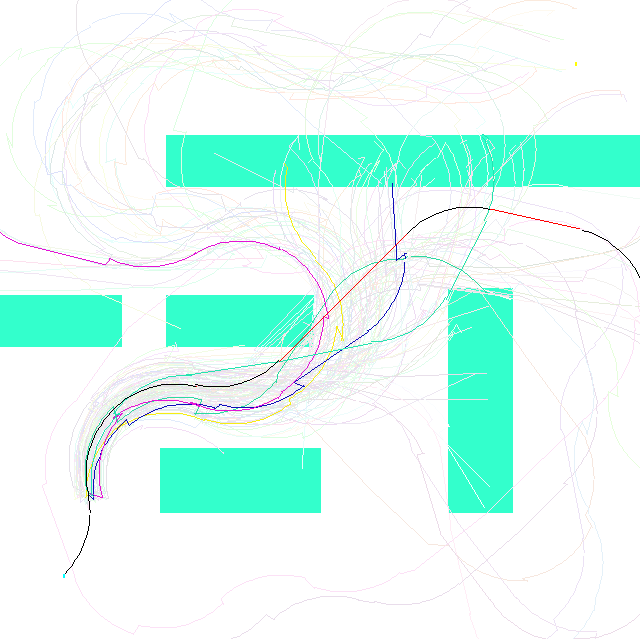
\includegraphics[width=5cm]{b_lowres.png}}
\end{figure}

\subsection{Effect of variance}

\subsection{Effect of reward}

\subsection{Effect of discount factor}

\section{Conclusion}
% * Briefly summarize your main findings.
We showed that the Markov Decision Process is able to give reasonable paths
to the robot even when the field is uncertain and constrainted heavily by
non-holonomic constraints.

\end{document}

